\section{Semaine 18 : 05/06/2023 - 09/06/2023}
\graphicspath{{semaines/semaine_18/images/}}

\begin{abstract}
	Lundi j'ai commencé à regarder comment appliquer la correction en $\mathbb{P}^{10}$ à partir de l'expression analytique obtenu par série de polynômes de Legendre. En fin de joournée, Emmanuel est passé et m'a expliqué une meilleure méthode pour calculer les coefficients des séries. 
	Dans la journée de mardi, j'ai pris le temps de trier les fichiers et mettre au propre tout le code. J'ai séparé les fonctions qui été toutes dans un même jupyter en différents fichiers pythons. J'ai également créé un fichyier de configuration "config.json" qui regroupe une partie des paramètres.
	Pour le reste de la semaine, j'ai implémenté et tester la nouvelle méthode pour calculer les coefficients de Legendre. J'ai commencé sur solution analytique 2D avec et sans changement de variables puis directement sur le FNO (sur $w$). Pour le FNO, j'ai considéré les mêmes erreurs que la semaine précédente en comparant $w$ et en comparant $u=\phi w$. On compare également errors\_legendre et errors\_FNO.
	En toute fin de semaine, j'ai également continué les tests sur la correction.
\end{abstract}

\subsection{Séparation des fichiers}

J'ai séparé le code en plusieurs modules, comme on peut le voir sur l'image de gauche. A droite, on peut voir les attributs et les fonctions de la classe \textbf{test\_sample\_legendre} :

\begin{minipage}{\linewidth}
	\centering
	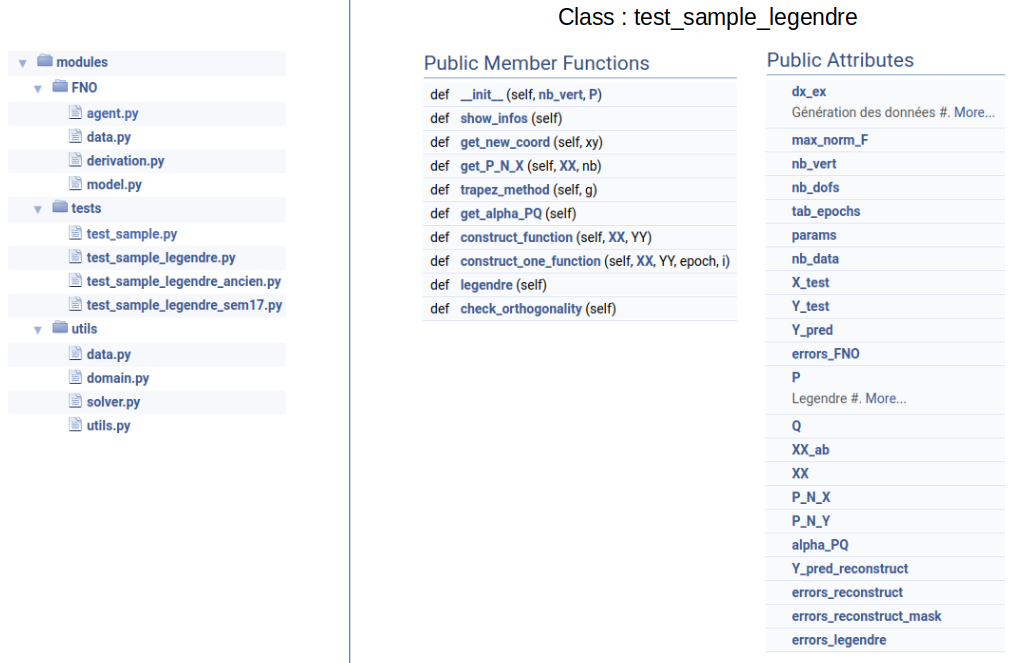
\includegraphics[width=0.78\linewidth]{tri_fichiers.png}
\end{minipage}

\begin{Rem}
	J'ai rapidement généré une documentation doxygen.
\end{Rem}

\subsection{Nouvelle méthode de calcul des coefficients de Legendre}

\begin{enumerate}[label=\textbullet]
	\item En 1D, on a 
	$$f(x)=\sum_{p=0}^{P-1}\alpha_p P_p(x)$$
	
	Ainsi pour tout $q=0,\dots,P-1$
	
	\begin{align*}
		\int_{-1}^1 f(x)P_q(x)dx &= \langle f,P_q\rangle_{L^2([-1,1])} \\
		&=\sum_{p=0}^{P-1}\alpha_p \langle P_p,P_q\rangle_{L^2([-1,1])} \\
		&=\alpha_q \langle P_q,P_q\rangle_{L^2([-1,1])} \\
	\end{align*}
	
	par orthogonalité des polynômes de Legendre dans $L^2([-1,1])$. 
	
	On en déduit
	
	$$\alpha_q = \frac{\langle f,P_q\rangle_{L^2([-1,1])}}{\langle P_q,P_q\rangle_{L^2([-1,1])}}=\frac{2q+1}{2}\langle f,P_q\rangle_{L^2([-1,1])}$$
	\item En 2D, on a
	$$f(x,y)=\sum_{p=0}^{P-1}\sum_{q=0}^{Q-1}\alpha_{p,q}P_p(x)P_q(y)$$
	Montrons dans un premier temps que les polynômes
	$$Q_{p,q}(x,y)=P_p(x)P_q(y)$$
	sont orthogonaux dans l'espace $L^2([-1,1]^2)$ :
	\begin{align*}
		\int_{-1}^1 \int_{-1}^1 Q_{p,q}(x,y)Q_{p',q'}(x,y)dxdy&=\int_{-1}^1 \int_{-1}^1 P_p(x)P_q(y)P_{p'}(x)P_{q'}(y)dxdy \\
		&=\int_{-1}^1 P_p(x)P_{p'}(x)dx\times \int_{-1}^1 P_q(y)P_{q'}(y)dy \\
		&=\frac{2}{2p+1}\delta_{pp'}\frac{2}{2q+1}\delta_{qq'} \\
		&=\frac{4}{(2p+1)(2q+1)}\delta_{(p,q)(p',q')}
	\end{align*}
	Ainsi pour tout $p'=0,\dots,P-1$,$q'=0,\dots,Q-1$
	
	\begin{align*}
		\int_{-1}^1 \int_{-1}^1 f(x,y)Q_{p',q'}(x,y)dxdy &= \langle f,Q_{p,q}\rangle_{L^2([-1,1]^2)} \\
		&=\sum_{p=0}^{P-1}\sum_{q=0}^{Q-1}\alpha_{p,q} \langle Q_{p,q},Q_{p',q'}\rangle_{L^2([-1,1]^2)} \\
		&=\alpha_{p',q'} \langle Q_{p',q'},Q_{p',q'}\rangle_{L^2([-1,1]^2)} \\
	\end{align*}
	
	par orthogonalité des polynômes $Q_{p,q}$ dans $L^2([-1,1]^2)$. 
	
	On en déduit
	
	$$\alpha_{p',q'} = \frac{\langle f,Q_{p',q'}\rangle_{L^2([-1,1]^2)}}{\langle Q_{p',q'},Q_{p',q'}\rangle_{L^2([-1,1]^2)}}=\frac{(2p'+1)(2q'+1)}{4}\langle f,Q_{p',q'}\rangle_{L^2([-1,1])}$$
	
	\begin{Rem}
		Pour calculer le produit scalaire sur $L^2([-1,1]^2)$, on va utiliser la méthode des trapèzes :
		\begin{align*}
			\int_{-1}^1\int_{-1}^1 g(x,y)dydx&=\int_{-1}^1\frac{2}{N-1}\sum_{i=0}^{N-1}\frac{g(x_i,y)+g(x_{i+1},y)}{2} \\
			&= \frac{1}{(N-1)^2}\sum_{i=0}^{N-1}\sum_{j=0}^{N-1}\left[g(x_i,y_i)+g(x_{i+1},y_i)+g(x_i,y_{i+1})+g(x_{i+1},y_{i+1})\right]
		\end{align*}
		ATTENTION : Il faut implémenter ce calcule de manière vectorielle sinon c'est beaucoup trop long (car double boucle sur $N$) :
\begin{lstlisting}
def trapez_method(self,g):
	N=self.nb_dofs
	sum_ij = g[:,:,:N-1,:N-1]+g[:,:,1:,:N-1]+g[:,:,:N-1,1:]+g[:,:,1:,1:]
	return 1/(N-1)**2 * np.sum(sum_ij,axis=(2,3))
\end{lstlisting}
		On utilisera également la fonction \href{https://numpy.org/doc/stable/reference/generated/numpy.polynomial.legendre.legval.html}{legval} de Numpy pour l'évaluation des polynômes de Legendre en nos degré de liberté.
	\end{Rem}
\end{enumerate}

\subsubsection{Résultats sur la solution analytique}

On prendra
$$u(x)=exp\left(-\frac{(x-\mu)^2+(y-\mu)^2}{2\sigma^2}\right)$$
avec $\mu=0$ et $\sigma=1$.
On prendra $P,Q=5$ et $N=100$.

On commence par vérifier l'orthogonalité des polynômes de Legendre :

\begin{minipage}{\linewidth}
	\centering
	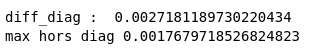
\includegraphics[width=0.3\linewidth]{ortho.png}
\end{minipage}

On testera également de faire varier $P$ et $N$.

\textbf{Sans changement de variable :}

En prenant $x\in[-1,1]$, voici les résultats obtenus pour epoch=0 et data=0 :

\begin{minipage}{\linewidth}
	\centering
	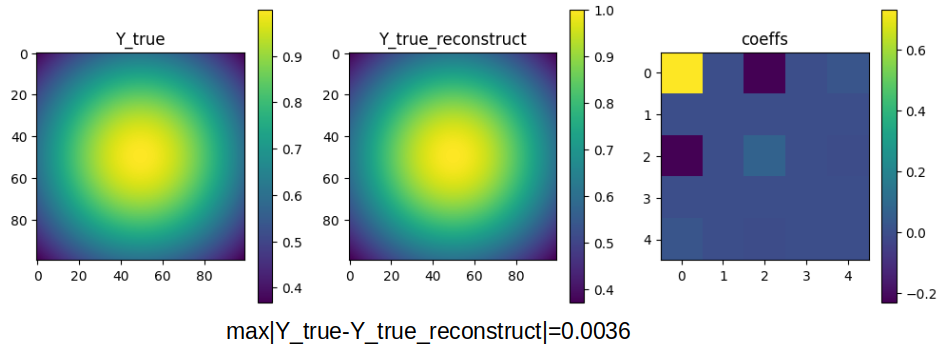
\includegraphics[width=0.6\linewidth]{example_P5.png}
\end{minipage}

Et en faisant varier $N$ et $P$ :

\begin{minipage}{\linewidth}
	\centering
	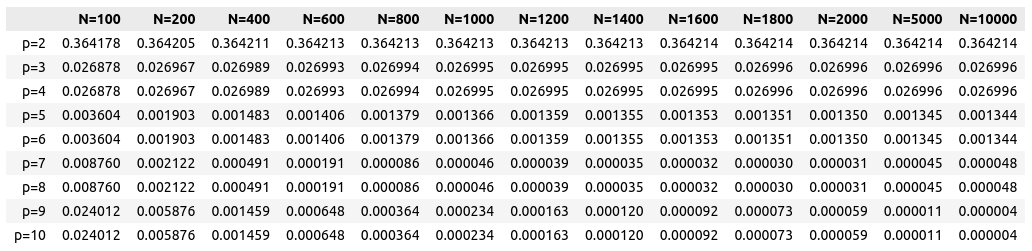
\includegraphics[width=0.9\linewidth]{varier_NP.png}
\end{minipage}

\textbf{Avec changement de variable :}

En prenant $x\in[0,1]$, voici les résultats obtenus pour epoch=0 et data=0 :

\begin{minipage}{\linewidth}
	\centering
	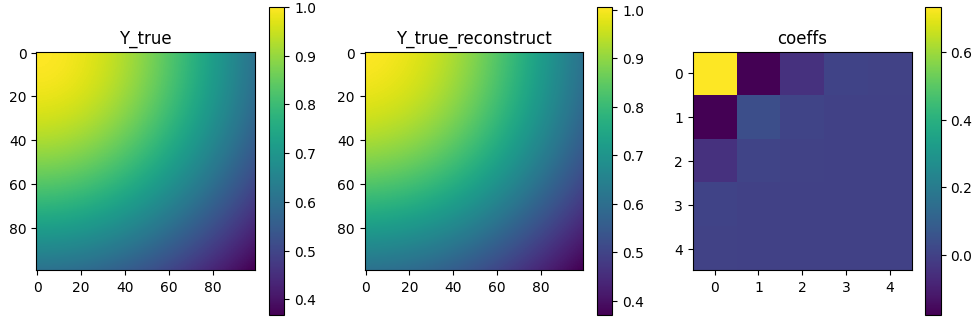
\includegraphics[width=0.6\linewidth]{example_P5_chgmt_vb.png}
\end{minipage}

Et en faisant varier $N$ et $P$ :

\begin{minipage}{\linewidth}
	\centering
	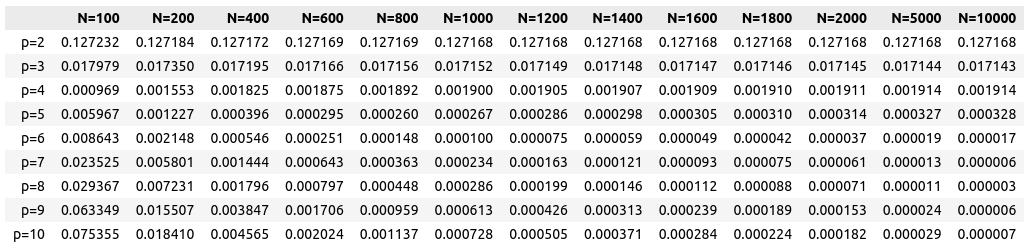
\includegraphics[width=0.9\linewidth]{varier_NP_chgmt_vb.png}
\end{minipage}

\subsubsection{Résultats sur le FNO}

On va régénérer les données en prenant
$$\alpha_{p,q}=\frac{(2p+1)(2q+1)}{4}\langle f,Q_{p,q}\rangle_{L^2([-1,1])}$$

De plus, on cherchera à décomposer en série de polynômes de Legendre la sortie du FNO (w) plutôt que la solution (c'est-à-dire la prédiction du FNO multipliée par la levelset $\phi$).

On considérera alors
$$w(x,y)=\sum_{p=0}^{P-1}\sum_{q=0}^{Q-1}\alpha_{p,q}P_p(x)P_q(y)$$

Ainsi
$$u(x,y)=w(x,y)\times\phi(x,y)$$

On considérera les cinq erreurs suivantes :
\begin{itemize}
	\item max(|Y\_pred-Y\_pred\_reconstruct|) -> errors\_reconstruct
	\item max(|(Y\_pred-Y\_pred\_reconstruct)*phi|) -> errors\_reconstruct\_phi
	\item max(|(Y\_pred-Y\_pred\_reconstruct)*mask|) -> errors\_reconstruct\_mask
	\item max(|(Y\_pred-Y\_pred\_reconstruct)*phi*mask|) -> errors\_reconstruct\_phi\_mask
	\item $||Y\_test-Y\_pred\_reconstruct||_{L^2}$  -> errors\_legendre
\end{itemize}

Pour $P=6$, voici les résultats obtenus :

\begin{minipage}{\linewidth}
	\centering
	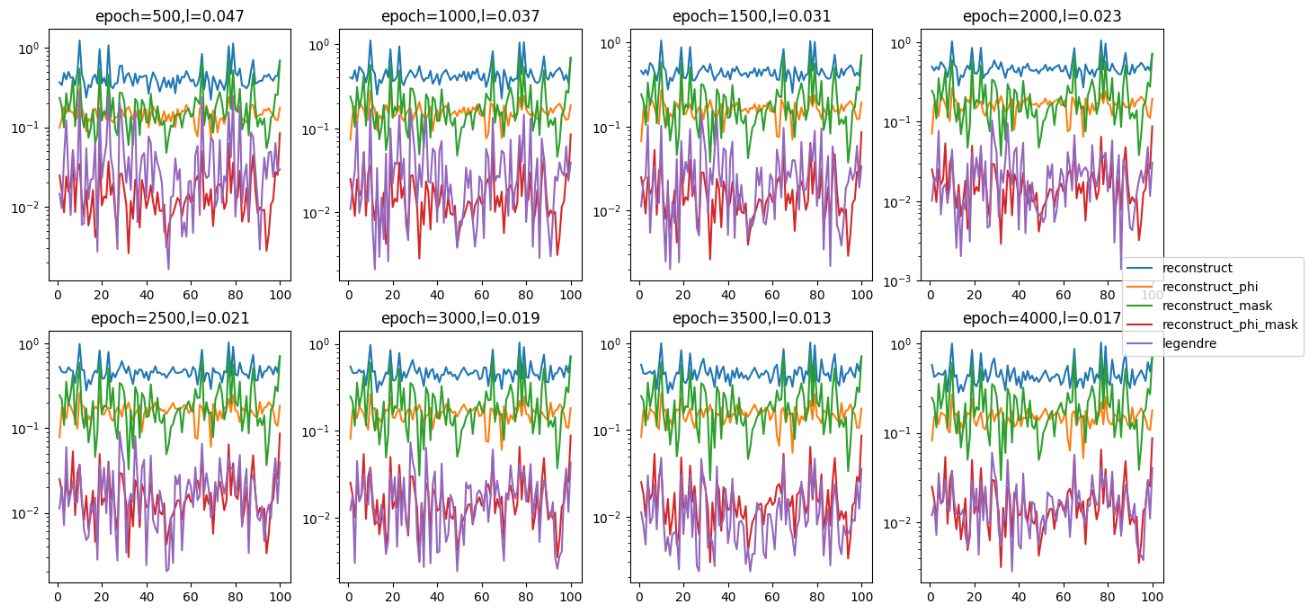
\includegraphics[width=0.9\linewidth]{FNO_errors5.png}
\end{minipage}

Pour epoch=0 et data=0, on a 

\begin{minipage}{\linewidth}
	\centering
	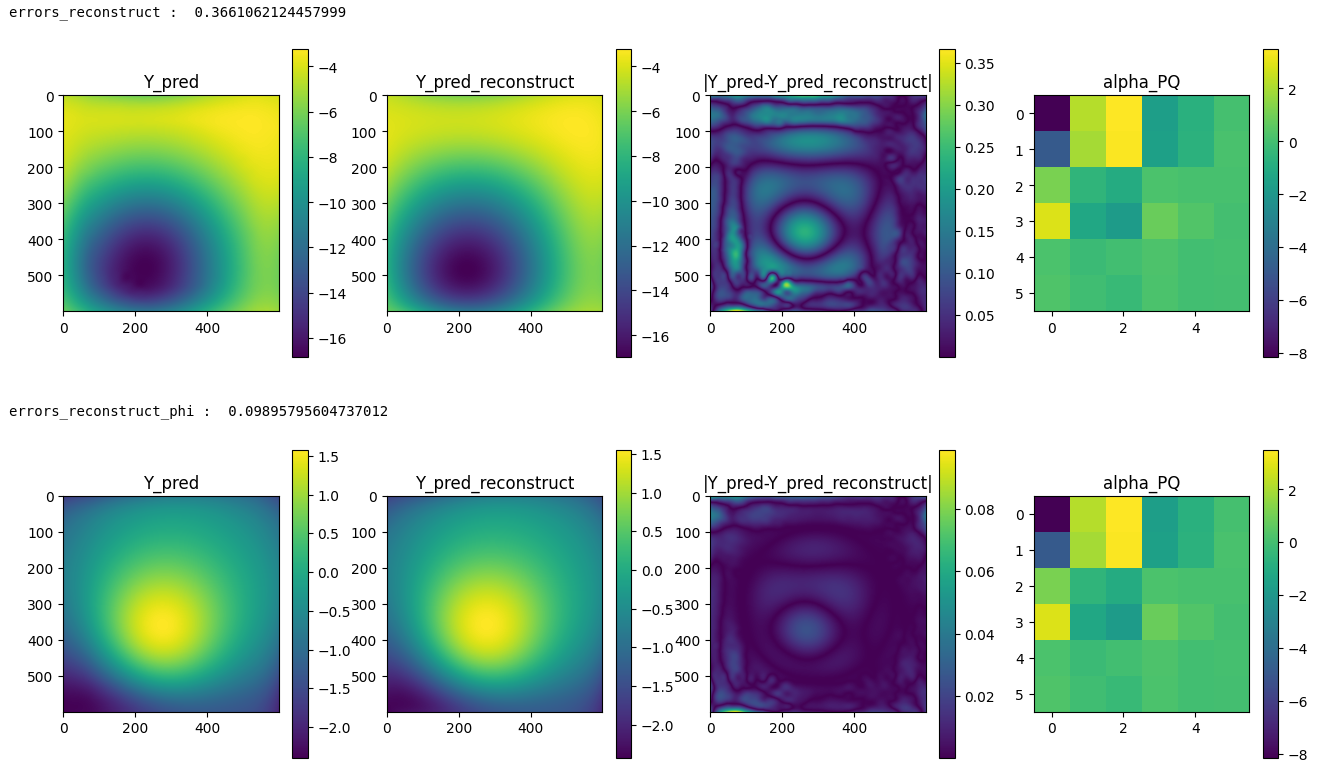
\includegraphics[width=0.9\linewidth]{FNO_example.png}
\end{minipage}

\begin{minipage}{\linewidth}
	\centering
	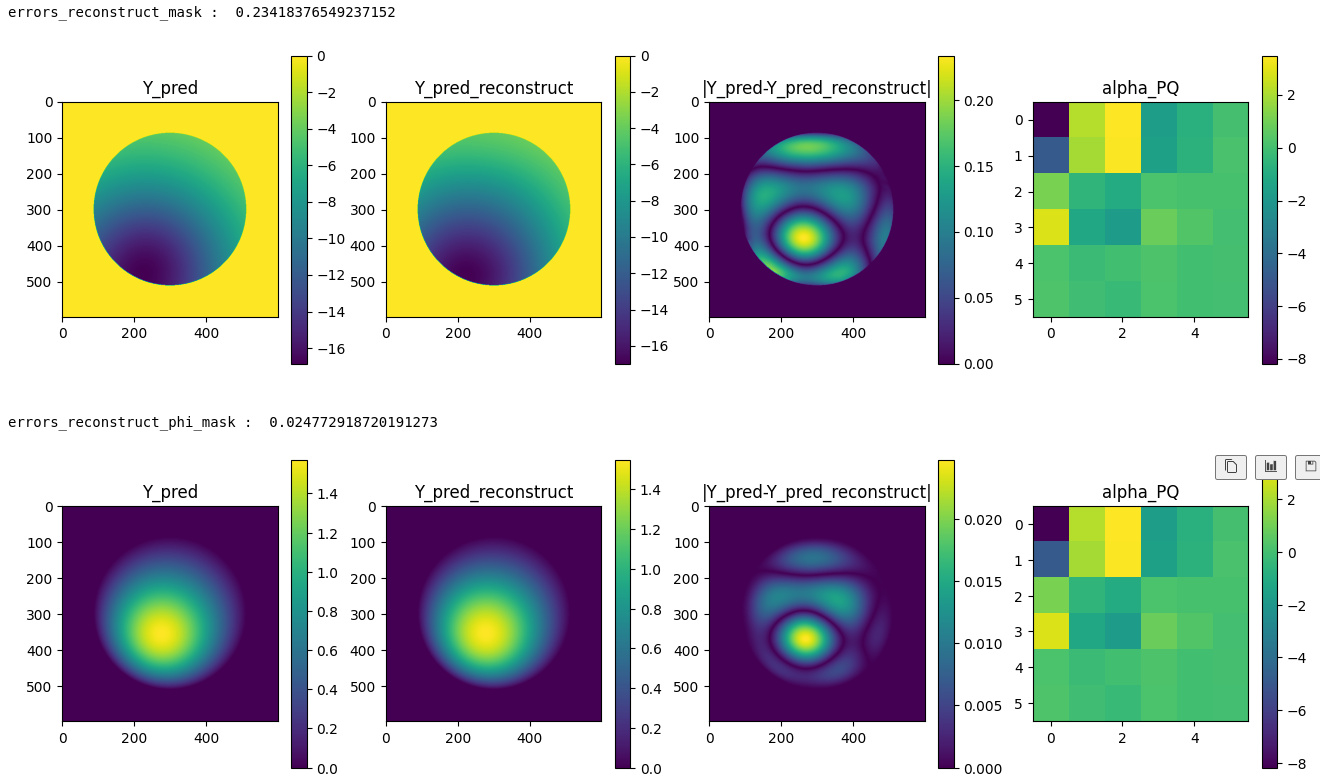
\includegraphics[width=0.9\linewidth]{FNO_example_mask.png}
\end{minipage}

En faisant varier $P$, on obtient les résultats suivants :

\begin{minipage}{\linewidth}
	\centering
	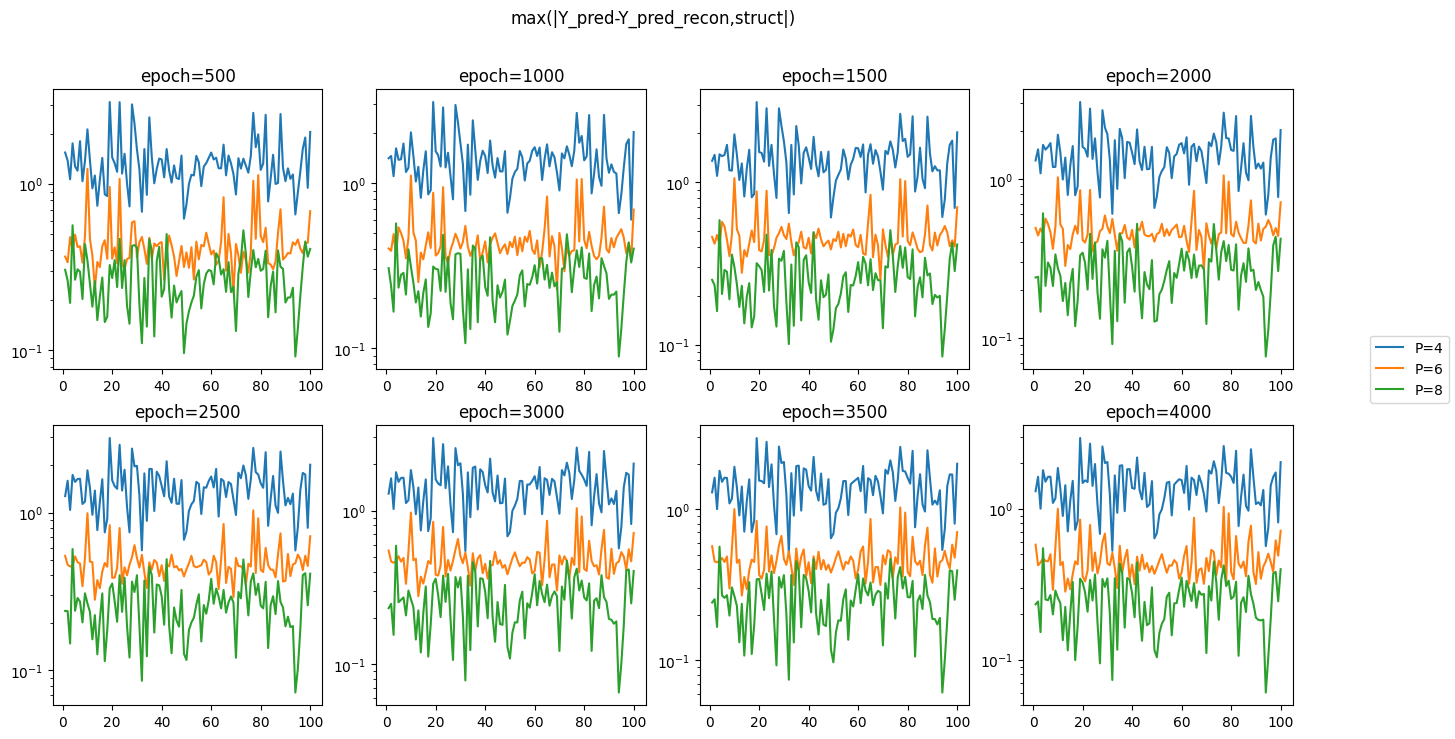
\includegraphics[width=0.8\linewidth]{FNO_varier_P_1.png}
\end{minipage}

\begin{minipage}{\linewidth}
	\centering
	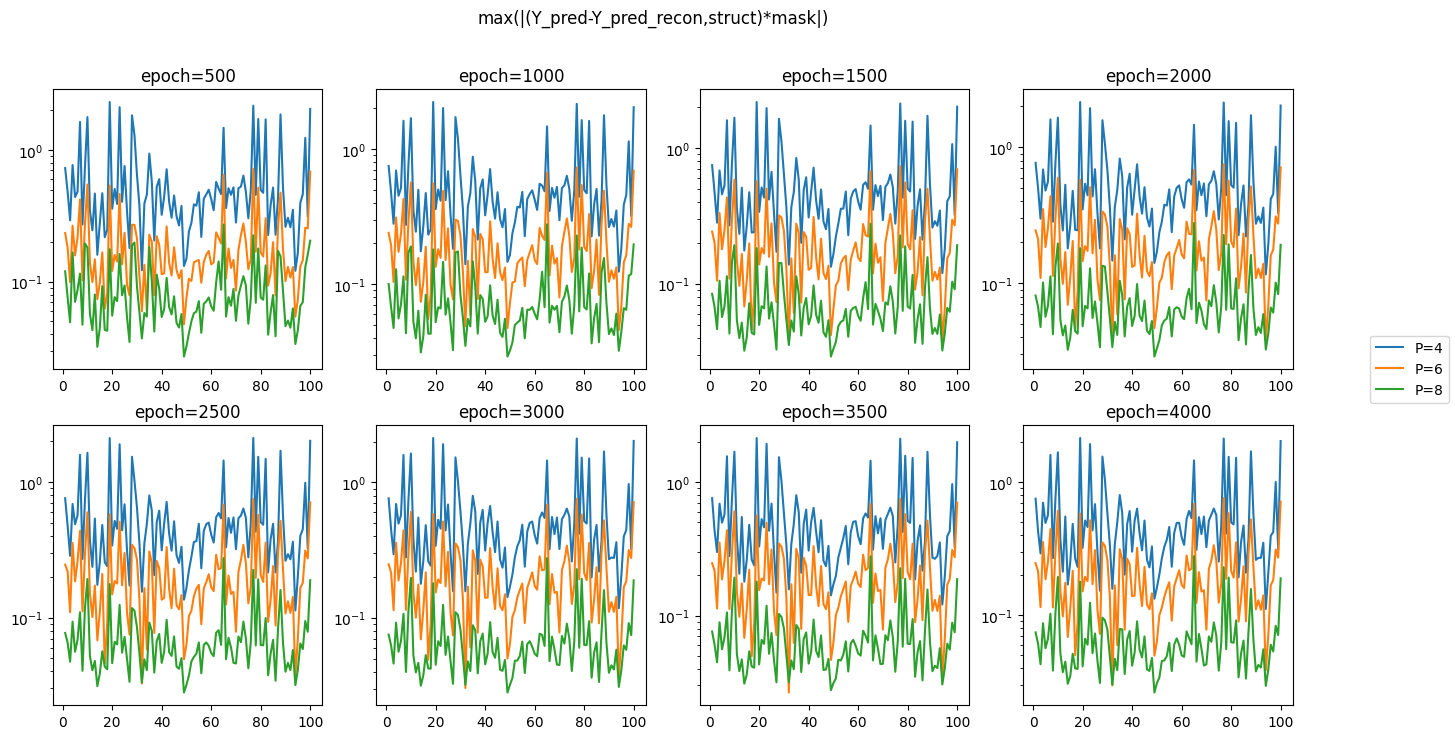
\includegraphics[width=0.8\linewidth]{FNO_varier_P_2.png}
\end{minipage}

\begin{minipage}{\linewidth}
	\centering
	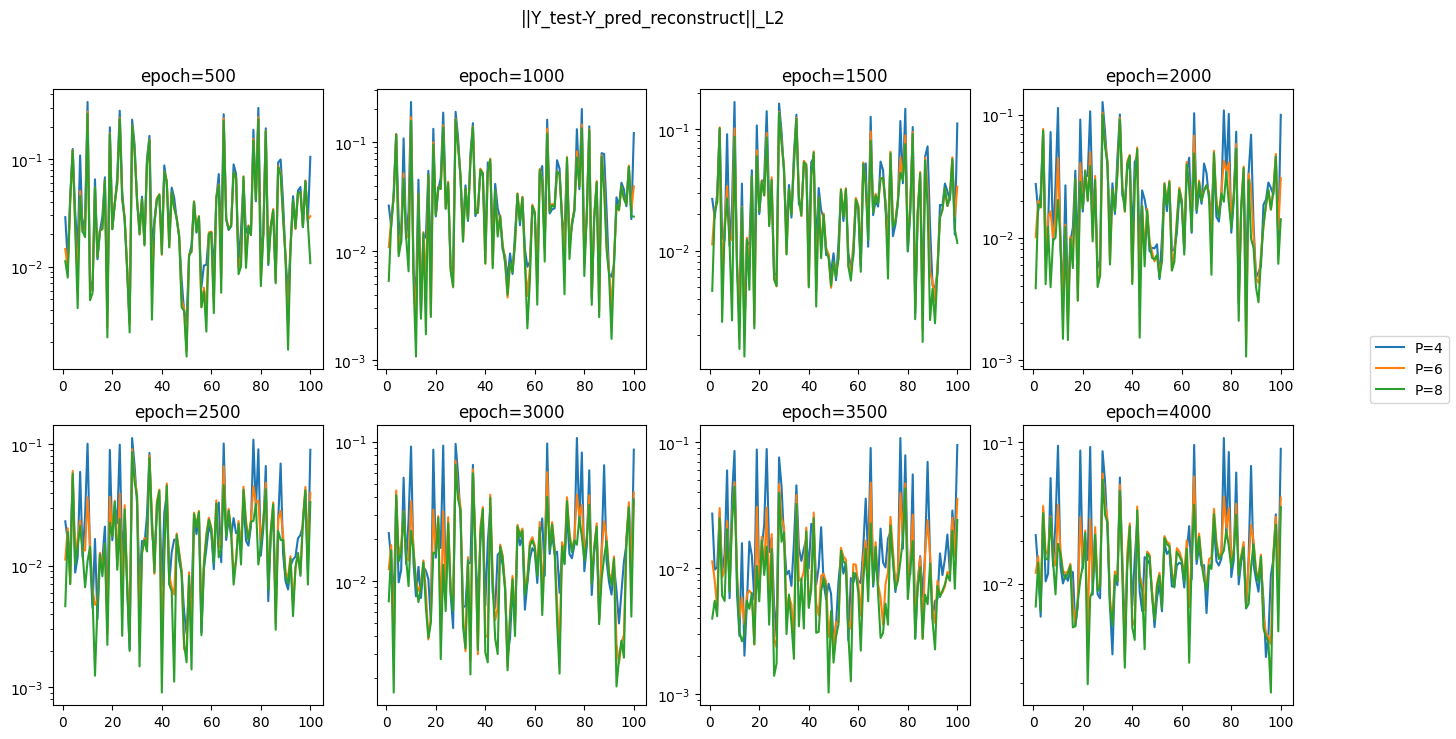
\includegraphics[width=0.8\linewidth]{FNO_varier_P_3.png}
\end{minipage}

\subsection{Correction de haut degré}

A ce stade, on a $\alpha_{p,q}$ pour chaque époque (sous-entendu celles enregistrées par le modèle) et pour chaque data. On souhaite appliquer les différents types de correction (par multiplication avec et sans rehaussement et par addition) en prenant 
$$\tilde{\phi}(x,y)=\left(\sum_{p=0}^{P-1}\sum_{q=0}^{Q-1}\alpha_{p,q} P_p(x)P_q(y)\right)\times \phi(x,y)$$

où $x,y$ sont les degrés de liberté associés à $\mathbb{P}^k$ avec $k$ assez grand (on aimerait prendre 10 par exemple).

On utilisera ensuite la fonction \textit{construct\_one\_function(XX,YY,epoch,data)} de la classe \textit{test\_sample\_legendre} qui pour une donnée évalue $\tilde{\phi}$ en les XX,YY. 

Dans le cas de correction où on utilisait directement la prédiction du FNO (multipliée par $\phi$), on récupérait la prédiction du FNO (dans $\mathbb{P}^2$) et à partir de celle-ci on générait une fonction FEniCS $\tilde{\phi}$ auquel on pouvait appliquer les différentes corrections. 

Dans le cas présent, on possède une expression analytique de la solution et donc il nous suffit de récupérer les degrés de liberté associés à $\mathbb{P}^k$ et d'évaluer $\tilde{\phi}$ en ces points.

Voici un exemple d'implémentation (pour $k=6$) :
\begin{lstlisting}
nb_vert = 300
P = 4
test_legendre = test_sample_legendre(nb_vert,P)

solver = CorrSolver(nb_cell=test_legendre.nb_vert-1, params=test_legendre.params, 
	Y_test=test_legendre.Y_test, V_ex=test_legendre.V_ex, dx_ex=test_legendre.dx_ex)

V_phi = FunctionSpace(solver.mesh,"CG",6)
XXYY = V_phi.tabulate_dof_coordinates().T
XX,YY = XXYY
XX = test_legendre.get_new_coord(XX)
YY = test_legendre.get_new_coord(YY)

epoch = 0
data = 5
f = test_legendre.construct_one_function(XX,YY,epoch,data)
f_FEniCS = Function(V_phi)
f_FEniCS.vector()[np.arange(0,f.shape[0],1)] = f
f_FEniCS = f_FEniCS * PhiExpr(degree=6,domain=solver.mesh)
\end{lstlisting}

\newpage

Voici les résultats obtenus (à gauche la solution prédite par le FNO pour nb\_vert=300 et à droite la solution FEniCS) :

\begin{minipage}{0.48\linewidth}
	\centering
	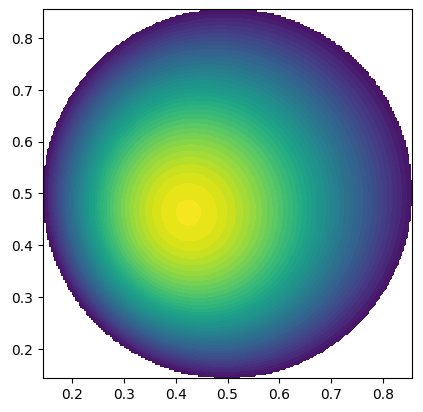
\includegraphics[width=0.6\linewidth]{corr_fenics.png}
\end{minipage}
\begin{minipage}{0.48\linewidth}
	\centering
	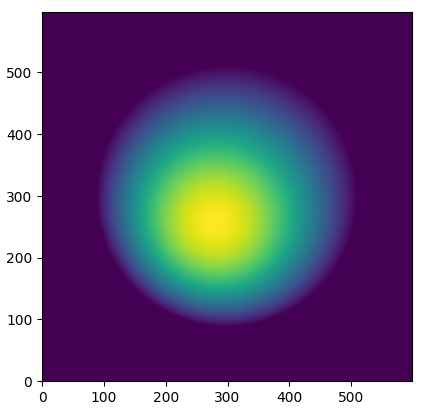
\includegraphics[width=0.6\linewidth]{corr_numpy.png}
\end{minipage}

\conclusion{Pour l'instant nous sommes bloqués ici car on n'a pas assez de RAM pour gérer d'aussi grosse résolution de problème variationnels. La semaine prochaine, il faudra effectués plusieurs tests dans le but de voir les limitations.}